\documentclass[12pt, oneside]{article}

\usepackage[letterpaper, scale=0.8, centering]{geometry}
\usepackage{fancyhdr}
\setlength{\parindent}{0em}
\setlength{\parskip}{1em}

\pagestyle{fancy}
\fancyhf{}
\renewcommand{\headrulewidth}{0pt}
\rfoot{{\footnotesize Copyright Daniel Grier / Mia Minnes, 2023, Version \today~(\thepage)}}

\usepackage{titlesec}

\author{CSE105Sp23}

\newcommand{\instructions}{{\bf For all HW assignments:} Weekly homework 
may be done individually or in groups of up to 3 students. 
You may switch HW partners for different HW assignments. 
The lowest HW score will not be included in your overall HW average. 
Please ensure your name(s) and PID(s) are clearly visible on the first page of your homework submission 
and then upload the PDF to Gradescope. If working in a group, submit only one submission per group: 
one partner uploads the submission through their Gradescope account and then adds the other group member(s) 
to the Gradescope submission by selecting their name(s) in the ``Add Group Members" dialog box. 
You will need to re-add your group member(s) every time you resubmit a new version of your assignment.
 Each homework question will be graded either for correctness (including clear and precise explanations and 
 justifications of all answers) or fair effort completeness. You may only collaborate on HW with CSE 105 students 
 in your group; if your group has questions about a HW problem, you may ask in drop-in help hours or post a private 
 post (visible only to the Instructors) on Piazza.

All submitted homework for this class must be typed. 
You can use a word processing editor if you like (Microsoft Word, Open Office, Notepad, Vim, Google Docs, etc.) 
but you might find it useful to take this opportunity to learn LaTeX. 
LaTeX is a markup language used widely in computer science and mathematics. 
The homework assignments are typed using LaTeX and you can use the source files 
as templates for typesetting your solutions.
To generate state diagrams of machines, we recommend using Flap.js
or JFLAP. Photographs of clearly hand-drawn diagrams may also be used. We recommend that you
submit early drafts to Gradescope so that in case of any technical difficulties, at least some of your
work is present. You may update your submission as many times as you'd like up to the deadline.


{\bf Integrity reminders}
\begin{itemize}
\item Problems should be solved together, not divided up between the partners. The homework is
designed to give you practice with the main concepts and techniques of the course, 
while getting to know and learn from your classmates.
\item You may not collaborate on homework with anyone other than your group members.
You may ask questions about the homework in office hours (of the instructor, TAs, and/or tutors) and 
on Piazza (as private notes viewable only to the Instructors).  
You \emph{cannot} use any online resources about the course content other than the class material 
from this quarter -- this is primarily to ensure that we all use consistent notation and
definitions (aligned with the textbook) and also to protect the learning experience you will have when
the `aha' moments of solving the problem authentically happen.
\item Do not share written solutions or partial solutions for homework with 
other students in the class who are not in your group. Doing so would dilute their learning 
experience and detract from their success in the class.
\end{itemize}

}

\newcommand{\gradeCorrect}{({\it Graded for correctness}) }
\newcommand{\gradeCorrectFirst}{\gradeCorrect\footnote{This means your solution 
will be evaluated not only on the correctness of your answers, but on your ability
to present your ideas clearly and logically. You should explain how you 
arrived at your conclusions, using
mathematically sound reasoning. Whether you use formal proof techniques or 
write a more informal argument
for why something is true, your answers should always be well-supported. 
Your goal should be to convince the
reader that your results and methods are sound.} }
\newcommand{\gradeComplete}{({\it Graded for completeness}) }
\newcommand{\gradeCompleteFirst}{\gradeComplete\footnote{This means you will 
get full credit so long as your submission demonstrates honest effort to 
answer the question. You will not be penalized for incorrect answers. 
To demonstrate your honest effort in answering the question, we ask 
that you include your attempt to answer *each* part of the question. 
If you get stuck with your attempt, you can still demonstrate 
your effort by explaining where you got stuck and what 
you did to try to get unstuck.} }

\usepackage{tikz}
\usetikzlibrary{automata,positioning,arrows}

\usepackage{amssymb,amsmath,pifont,amsfonts,comment,enumerate,enumitem}
\usepackage{currfile,xstring,hyperref,tabularx,graphicx,wasysym}
\usepackage[labelformat=empty]{caption}
\usepackage{xcolor}
\usepackage{multicol,multirow,array,listings,tabularx,lastpage,textcomp,booktabs}

\lstnewenvironment{algorithm}[1][] {   
    \lstset{ mathescape=true,
        frame=tB,
        numbers=left, 
        numberstyle=\tiny,
        basicstyle=\rmfamily\scriptsize, 
        keywordstyle=\color{black}\bfseries,
        keywords={,procedure, div, for, to, input, output, return, datatype, function, in, if, else, foreach, while, begin, end, }
        numbers=left,
        xleftmargin=.04\textwidth,
        #1
    }
}
{}

\newcommand\abs[1]{\lvert~#1~\rvert}
\newcommand{\st}{\mid}

\newcommand{\cmark}{\ding{51}}
\newcommand{\xmark}{\ding{55}}
 
\newcommand{\SUBSTRING}{\textsc{Substring}}
\newcommand{\REP}{\textsc{Rep}}
\newcommand{\blank}{\scalebox{1.5}{\textvisiblespace}}
 
\title{HW6 : Computational Problems, Recognizability, Decidability}
\date{Due: May 23th at 5pm (no penalty late submission until 8am next morning), via Gradescope}

\begin{document}
\maketitle
\thispagestyle{fancy}

\textbf{In this assignment:} You will use general constructions and specific machines 
to explore the classes of recognizable and decidable languages. You will explore various 
ways to encode machines as strings so that computational problems can be recognized.

\textit{Resources}:  To review the topics you are working with for this assignment, 
see the class material from Week 6 through Week 7. We will post frequently asked questions 
and our answers to them in a pinned Piazza post.

\textit{Reading and extra practice problems}: Chapter 4 exercises 4.1, 4.3, 4.4., 4.5. 
Chapter 4 Problems 4.29, 4.30.

\textit{Key Concepts:} uring-recognizable languages, Turing-decidable languages, 
Church-Turing thesis, computational problems.

\instructions

You will submit this assignment via Gradescope
(\href{https://www.gradescope.com}{https://www.gradescope.com}) 
in the assignment called ``hw6CSE105Sp23''.

\textbf{Assigned questions}

\begin{enumerate} 
\item \textbf{Explicit encodings} (8 points): \\
In a computational problem, the elements of the language are encodings of machines. For example, 
consider the language 
\[
E_{\mathrm{DFA}} := \{ \langle M \rangle \mid M \text{ is a DFA, and } L(M) = \varnothing \}
\]
where each string $\langle M \rangle$ in the language encodes a DFA $M = (Q, \Sigma, \delta, q_0, F)$.
Usually, we purposefully drop the details about how this encoding is done because they can distract from 
the central computational 
properties of the language. In fact, any encoding can be used so long as there exists a decider for 
syntactic questions about the DFAs being encoded. 
In this question, we will build some specific 
explicit examples of encodings of DFAs to get more comfortable with these ideas.

\begin{enumerate}
\item\gradeCompleteFirst \textit{Encoding with delimiters:} Perhaps the most straightforward
way to create an encoding is to have it mirror the structure of the tuple $(Q, \Sigma, \delta, q_0, F)$ 
for the DFA. Your task: describe an encoding that maps each DFA $M$ to a distinct string $\langle M \rangle$ 
that uniquely identifies $M$. That is, if you ``decode'' the encoding, you get the exact same machine back. 

\noindent{\it Hints, tips, notes of caution:}
\begin{itemize}[itemsep=-10pt]
\item You may use special characters like $\#$ and $\$$ as delimiters in your encoding to separate the 
various components. \\
\item Your encoding alphabet must be finite
\end{itemize}
\item\gradeComplete Use your encoding from part (a) to produce
the string encoding the DFA below:
\begin{center}
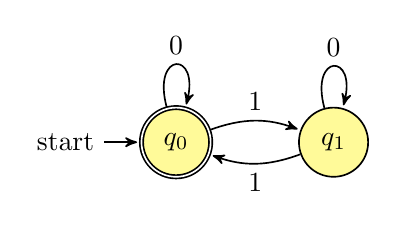
\begin{tikzpicture}[->,>=stealth',shorten >=1pt, auto, node distance=2cm, semithick]
  \tikzstyle{every state}=[text=black, fill=yellow!40]

  \node[initial,state, accepting] (q0)                    {$q_0$};
  \node[state]         (q1) [right of=q0] {$q_1$};

  \path (q0) edge  [loop above] node {$0$} (q0)
  		edge [bend left=20] node {$1$} (q1)
	(q1) edge [loop above] node {$0$} (q1)
		edge [bend left=20] node {$1$} (q0)
 ;
\end{tikzpicture}
\end{center}

\item\gradeComplete Show that it is possible to have the same kind of delimited encoding without 
using special delimiter characters. In particular, prove that for every DFA $M$, 
we can assume that $\langle M \rangle \subseteq \{0,1\}^*$.

\end{enumerate}

\noindent\textit{Challenge; not graded:\newline For the delimited encoding schemes above, 
there are strings over the encoding alphabet 
($\Sigma$) that nevertheless do not correspond to a valid DFA. \newline \newline
Prove/disprove: There exists an encoding scheme for which this is not true; that is, 
\[\{ \langle M \rangle \mid M \text{ is a DFA}\} = \Sigma^*.\]}

\vfill



\item \textbf{Closure} (18 points): \\
Let $\Sigma = \{0,1\}$ and $\Gamma = \{0,1,2\}$. Recall the functions
    \begin{align*}
    \SUBSTRING(K) &:= \{ w \in \Gamma^* \mid \text{there exist } a,b \in \Gamma^* \text{ such that } awb \in K\} \\
    \REP(L) &:= \{ w \in \Gamma^* \mid \text{between every 
    pair of successive $2$s in $w$ is a string in $L$}\}\\
    &\phantom{:}=\{w \in \Gamma^* \mid \text{for all } v \in \Sigma^* \text{ if } 2v2 \in \SUBSTRING(\{w\})  \text{, then } v \in L\}
    \end{align*}
\begin{enumerate}
    \item\gradeCorrectFirst Prove that, given any deterministic decider
    over $\Sigma$, $M_L$, there is a deterministic decider over 
    $\Gamma$ that recognizes $$\REP(~L(M_L)~)$$
    In other words, you 
    will prove that for any Turing-decidable language $L$ over $\Sigma$, 
    $\REP(L)$
    is also Turing-decidable. A complete answer will 
    include both a precise construction of the machine and a 
    (brief) justification of why this machine works as required.
    
    \item\gradeCorrect Prove that, given any nondeterministic Turing machine over 
    $\Gamma$, $N_L$, there is a nondeterministic Turing machine over 
    $\Gamma$ that recognizes $$\SUBSTRING(~L(N_L)~)$$
    In other words, you will prove that the class of Turing-recognizable languages 
    over $\Gamma$ is closed 
    under the $\SUBSTRING$ operation.
     A complete answer will 
    include both a precise construction of the machine and a 
    (brief) justification of why this machine works as required.
    
    \item\gradeComplete Give a different proof that the class of Turing-recognizable 
    languages over $\Gamma$ is closed 
    under the $\SUBSTRING$ operation, this time using only deterministic Turing machines.  A complete answer will 
    include both a precise construction of the machine and a 
    (brief) justification of why this machine works as required.

\end{enumerate}


\item \textbf{Computational problems} (24 points): \\
For each of the following statements, determine if it is true or false. 
Clearly label your choice 
by starting your solution with {\bf True} or {\bf False} and then
provide a brief (3-4 sentences or so) justification for your answer.

\begin{enumerate}
\item\gradeCorrect For each regular language $K$, the language 
\[
\{ \langle M \rangle \mid M \text{ is a DFA and } L(M) = K\} 
\]
is decidable.

\item\gradeCorrect For each regular language $L$, the language
\[
\{ \langle M_1, M_2 \rangle \mid M_1, M_2\text{ are both DFA and } 
L(M_1) \subseteq L \text{ and } L(M_2) \subseteq \overline{L}\}
\]
is decidable.


\item\gradeCorrect Let $\mathrm{Model} \in \{\mathrm{DFA}, \mathrm{NFA}, 
\mathrm{REX}, \mathrm{CFG}, \mathrm{PDA} \}$. If $EQ_{\mathrm{Model}}$ is decidable, 
then $E_{\mathrm{Model}}$ is decidable.

\end{enumerate}

{\it Challenge; not graded: Let $\mathrm{Model} \in \{\mathrm{DFA}, \mathrm{NFA}, 
\mathrm{REX}, \mathrm{CFG}, \mathrm{PDA} \}$. If $A_{\mathrm{Model}}$ is decidable, 
then $EQ_{\mathrm{Model}}$ is decidable.}

\end{enumerate}

\end{document}